\chapter{Kardinalite ve Sonsuzluk}
\label{chap:kardinalite}


\par\smallskip{\sffamily\bfseries\color{cAcc}Öğrenme Hedefleri}\nopagebreak

\begin{itemize}\setlength{\itemsep}{2pt}\setlength{\parskip}{0pt}
\item Eş güçlülüğü eşleme üzerinden tanımlayabilme.
\item ℕ, ℤ, ℚ’nün sayılabilir, ℝ’nin sayılamaz olduğunu gerekçelendirebilme.
\item Sonlu–sonsuz ayrımının felsefi boyutunu tartışabilme.
\end{itemize}

\section*{Bölüme Genel Bakış: Sonsuzu Saymak}

Sonsuzluk, matematiğin en eski ve en sarsıcı kavramıdır. Galileo, on yedinci yüzyılda tam karelerin (1, 4, 9, …) tüm doğal sayılarla birebir eşlenebildiğini fark etti; ‘parça, bütün kadar çok’ görünüyordu ve bu sezgiyle çeliştiği için Galileo, sonsuzların karşılaştırılamayacağı sonucuna vardı. İki yüzyıl sonra Bernard Bolzano bu paradoksları yeniden ele aldı; ama asıl atılımı Georg Cantor yaptı: 1874 ve 1891’de sonsuz kümelerin farklı ‘büyüklüklere’ sahip olabileceğini kesin biçimde kanıtladı. Richard Dedekind ise sonsuz kümeyi tam da bu şaşırtıcı özellikle tanımladı: bir küme, öz bir alt kümesiyle eş güçlüyse sonsuzdur.

Bu bölüm, sonsuzu bir sezgi olmaktan çıkarıp üzerinde kesin teoremler kanıtlanan bir nesneye dönüştüren Cantor programını izler. Eş güçlülük, sayılabilirlik ve köşegen argümanı aracılığıyla ‘bazı sonsuzların diğerlerinden büyük olduğu’ sonucuna varırız. Öğretmen adayı için bu konu, hem matematiksel titizliğin zaferini hem de sezginin sınırlarını bir arada gösteren güçlü bir örnektir ve dersin tüm teknik omurgasını bir doruğa taşır.

\section{Eş Güçlülük}

\begin{tcolorbox}[bookbox,colback=cDef]\textbf{\textsf{\textcolor{cAcc}{Tanım.}}}\quad A ile B eş güçlüdür (|A| = |B|), aralarında bir eşleme varsa. Bir küme sayılabilir sonsuzdur, ℕ ile eş güçlüyse; sayılamazdır, sonsuz olup ℕ ile eş güçlü değilse.\end{tcolorbox}

\section{Sayılabilir Kümeler}

ℤ sayılabilirdir: 0, 1, −1, 2, −2, … sıralaması ℕ ile bir eşleme verir. ℚ da sayılabilirdir; kesirler bir tablo hâlinde dizilip köşegen yöntemiyle tek sıraya konabilir. Bu, ‘sonsuzun sonsuzu’ görünen ℚ’nün aslında ℕ kadar çok olduğunu gösterir.

\section{ℝ Sayılamaz: Cantor Köşegeni}

Köşegen argümanı tarihsel olarak küme kuramı paradokslarına giden yolun da bir durağıdır: Russell, paradoksuna Cantor’un ‘en büyük kardinal yoktur’ ispatını incelerken ulaşmıştır. Bu bölümde aynı fikri ondalık açılımlar üzerinde tam bir ispat olarak yazıyor ve eş güçlülüğün genel kuramına yerleştiriyoruz.

\begin{tcolorbox}[bookbox,colback=cDef]\textbf{\textsf{\textcolor{cAcc}{Teorem.}}}\quad (0, 1) aralığı sayılamazdır.\end{tcolorbox}

\begin{tcolorbox}[bookbox,colback=cEx]\textbf{\textsf{\textcolor{cAcc}{Örnek.}}}\quad İspat fikri (köşegen): (0,1)’in sayılabilir olduğunu, yani tüm ondalık açılımların bir listeye dizildiğini varsayalım. Köşegendeki i’nci basamağı değiştirerek yeni bir d sayısı kuralım (her basamağı listedeki i’nci sayının i’nci basamağından farklı seçelim). d, listedeki her sayıdan en az bir basamakta farklı olduğundan listede yer alamaz — çelişki. Öyleyse böyle bir liste yoktur; (0,1) sayılamaz. ∎\end{tcolorbox}

Aynı köşegen fikri genelleşir: her A kümesi için |A| < |P(A)| (Cantor teoremi). Böylece sonsuzun tek bir büyüklüğü değil, sonsuz bir hiyerarşisi vardır.

\begin{tcolorbox}[bookbox,colback=cDep]\textbf{\textsf{\textcolor{cAcc}{Muhakeme/Felsefe Derinleştirmesi — Edimsel ve olası sonsuzluk; Hilbert Oteli}}}\quad Aristo’dan beri süregelen ayrım, sonsuzun ‘tamamlanmış bir bütün’ (edimsel) mi yoksa yalnızca ‘hep daha ileri gidebilme’ (olası) mi olduğudur. Cantor’un eş güçlülük kuramı, edimsel sonsuzu matematiğin meşru bir nesnesi hâline getirdi — ve bu, dersin başında gördüğümüz temellendirme bunalımlarının merkezindeydi. Hilbert’in ‘sonsuz odalı oteli’ (dolu otel yeni konuğu, hatta sonsuz konuğu ağırlayabilir), sayılabilir sonsuzun sonlu sezgiyi nasıl kırdığını gösterir. Süreklilik hipotezi — ℕ ile ℝ arasında bir kardinalite olup olmadığı — ise ZFC’den bağımsızdır: aksiyomatik yöntemin sınırlarına dair somut bir örnektir.\end{tcolorbox}

\begin{figure}[htbp]
\centering
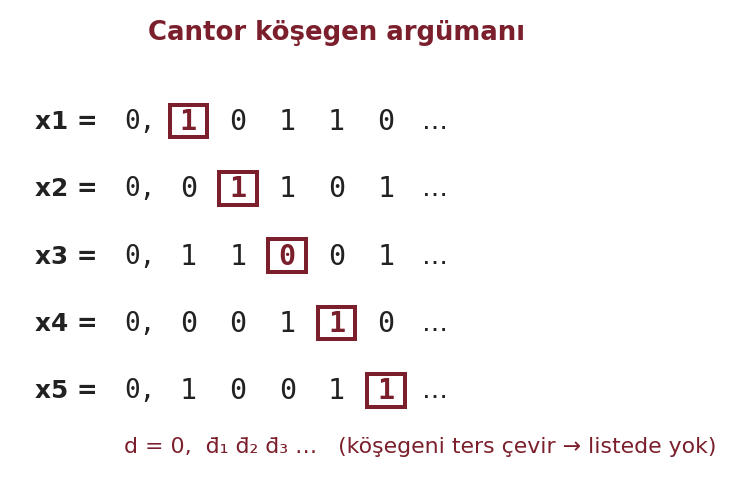
\includegraphics[width=0.80\linewidth]{figs/cantor.png}
\caption{Cantor köşegen argümanı: köşegen değiştirilerek listede olmayan bir sayı kurulur.}
\end{figure}

\section{İleri Örnekler: Eşlemeler ve Köşegen}

Sonsuz kümeleri karşılaştırmak, somut eşlemeler kurmayı ve köşegen argümanını ayrıntılı izlemeyi gerektirir. Aşağıdaki örnekler sayılabilirliğin sınırını ve sayılamazlığın kanıtını netleştirir.

\begin{tcolorbox}[bookbox,colback=cEx]\textbf{\textsf{\textcolor{cAcc}{Örnek.}}}\quad \textbf{Aralık ile tüm doğru eş güçlüdür. }f: (0, 1) → ℝ, f(x) = tan(π(x − ½)) bir eşlemedir: x, 0’dan 1’e giderken π(x − ½) açısı −π/2’den π/2’ye gider ve tan bu aralıkta tüm ℝ’yi birebir tarar. Demek ki minik bir açık aralık, tüm gerçel doğruyla aynı ‘büyüklüktedir’ — sonsuzda uzunluk sezgisi çöker.\end{tcolorbox}

\begin{tcolorbox}[bookbox,colback=cEx]\textbf{\textsf{\textcolor{cAcc}{Örnek.}}}\quad \textbf{ℚ sayılabilirdir. }Pozitif kesirler p/q, satırları pay ve sütunları payda olan sonsuz bir tabloya yerleştirilip köşegenler boyunca (tekrarları atlayarak) tek bir diziye dizilebilir: 1/1, 2/1, 1/2, 1/3, 2/2(atlanır), 3/1, … Negatifler ve sıfır da araya serpiştirilince ℚ ile ℕ arasında bir eşleme elde edilir. ‘Yoğun’ görünen ℚ, aslında ℕ kadar çoktur.\end{tcolorbox}

\begin{tcolorbox}[bookbox,colback=cEx]\textbf{\textsf{\textcolor{cAcc}{Örnek.}}}\quad \textbf{Köşegen argümanı (ayrıntılı). }(0, 1)’in sayılabilir olduğunu, yani tüm ondalık açılımların x₁, x₂, x₃, … diye listelendiğini varsayalım. Her xᵢ’nin i’nci ondalık basamağını değiştirerek yeni bir d = 0,d₁d₂d₃… sayısı kuralım (dᵢ, xᵢ’nin i’nci basamağından farklı; 0 ve 9’dan kaçınarak). d, listedeki her sayıdan en az bir basamakta ayrıldığından listede yer alamaz — oysa d ∈ (0, 1). Çelişki; demek ki böyle bir liste yoktur ve (0, 1) sayılamazdır. ∎\end{tcolorbox}

\begin{tcolorbox}[bookbox,colback=cEx]\textbf{\textsf{\textcolor{cAcc}{Örnek.}}}\quad \textbf{|P(ℕ)| = |ℝ|. }Her gerçel sayının ikili açılımı bir 0–1 dizisidir; her 0–1 dizisi de ℕ’nin bir alt kümesini (1 gelen konumların kümesi) belirler. Bu, ℝ ile P(ℕ) arasında (küçük teknik düzeltmelerle) bir eşleme verir. Cantor teoremi |ℕ| < |P(ℕ)| olduğundan, ℝ’nin ℕ’den kesinlikle ‘daha büyük’ bir sonsuz olduğunu bir kez daha görürüz.\end{tcolorbox}

\begin{tcolorbox}[bookbox,colback=cEx]\textbf{\textsf{\textcolor{cAcc}{Örnek.}}}\quad \textbf{Cantor–Schröder–Bernstein teoremi. }A’dan B’ye ve B’den A’ya birer birebir fonksiyon varsa, A ile B arasında bir eşleme vardır: |A| ≤ |B| ve |B| ≤ |A| ⇒ |A| = |B|. Bu teorem, iki yönde birebirlik göstererek eş güçlülüğü kanıtlamayı — açık bir eşleme kurmadan — mümkün kılar; kardinalite karşılaştırmasının ‘antisimetri’ özelliğidir.\end{tcolorbox}

\begin{tcolorbox}[bookbox,colback=cMis]\textbf{\textsf{\textcolor{cAcc}{Yaygın Kavram Yanılgıları}}}\quad \textbf{“Tüm sonsuz kümeler aynı büyüklüktedir.” — }Hayır; ℕ sayılabilir, ℝ sayılamazdır. Cantor teoremi sonsuz büyüklüklerin bir hiyerarşisi olduğunu gösterir.\par\medskip{}\textbf{“Sonsuz + sonsuz daha büyük bir sonsuz verir.” — }Sayılabilir iki kümenin birleşimi yine sayılabilirdir; ℤ = negatifler ∪ \{0\} ∪ pozitifler hâlâ ℕ kadardır.\par\medskip{}\textbf{“ℚ, ℝ içinde yoğun olduğundan onunla aynı boyuttadır.” — }Yoğunluk kardinalite demek değildir; ℚ sayılabilir, ℝ sayılamazdır.\par\medskip{}\textbf{“0,999… sayısı 1’den küçüktür.” — }0,999… = 1’dir; aradaki fark her ondalık basamakta 0’dır. Bu, sonsuz süreçlerin sonlu sezgiyle çeliştiği tipik bir noktadır.\par\medskip{}\textbf{“Sayılabilir sonsuz, sonlu gibi davranır.” — }Aksine: bir sonsuz küme öz alt kümesiyle eş güçlü olabilir (çift sayılar ↔ ℕ), ki bu sonlu kümelerde imkânsızdır.\end{tcolorbox}

\section{Uygulama ve Eğitime Yansıma}

Kardinalite, hesaplanabilirlik kuramının kalbindedir. Yazılabilecek tüm bilgisayar programları sonlu birer metin olduğundan sayılabilir çokluktadır; oysa ℕ’den \{0,1\}’e fonksiyonlar sayılamaz çokluktadır. Sayılabilir çok program ile sayılamaz çok fonksiyon karşılaştırıldığında kaçınılmaz sonuç şudur: hiçbir programın hesaplayamayacağı fonksiyonlar vardır. Böylece Cantor’un köşegen fikri, doğrudan Turing’in hesaplanamazlık sonuçlarına ve durma probleminin çözülemezliğine bağlanır.

Eğitim açısından sonsuzluk, öğrencinin sonlu sezgisiyle en sert çatışan konudur; bu yüzden dikkatle ele alınmalıdır. Hilbert’in sonsuz odalı oteli, ‘dolu’ bir otelin yeni (hatta sonsuz sayıda) konuğu nasıl ağırlayabileceğini canlandıran güçlü bir sınıf etkinliğidir ve öğrenciyi ‘bütün ile parçanın eş güçlü olabileceği’ fikrine hazırlar. Öğretmenin görevi, bu şaşırtıcı sonuçları birer paradoks olarak değil, eş güçlülük tanımının tutarlı sonuçları olarak sunmaktır.

\section{Yüksek Lisans Derinleştirmesi: Alefler ve Süreklilik Hipotezi}

Cantor, sonsuz büyüklükleri ‘alef’ sayılarıyla adlandırdı: sayılabilir sonsuzun kardinalitesi ℵ₀, gerçel sayılarınki ise 2\textasciicircum{}\{ℵ₀\} (‘süreklinin gücü’) olarak gösterilir. Cantor teoremi |A| < |P(A)| her küme için geçerli olduğundan, ℵ₀ < 2\textasciicircum{}\{ℵ₀\} < 2\textasciicircum{}\{2\textasciicircum{}\{ℵ₀\}\} < … biçiminde sonsuza dek yükselen bir büyüklükler hiyerarşisi doğar. Sonsuz, tek bir kavram değil, uçsuz bucaksız bir merdivendir.

Süreklilik hipotezi (CH), ℵ₀ ile 2\textasciicircum{}\{ℵ₀\} arasında başka bir kardinalitenin bulunup bulunmadığını sorar; yani ℕ’den büyük, ℝ’den küçük bir sonsuz var mıdır? Cantor bunun olmadığını (2\textasciicircum{}\{ℵ₀\} = ℵ₁) savundu ama kanıtlayamadı. Sonuç şaşırtıcıdır: Kurt Gödel (1940) CH’nin ZFC ile çelişmediğini, Paul Cohen (1963, ‘forcing’ yöntemiyle) CH’nin olumsuzunun da ZFC ile çelişmediğini gösterdi. Yani CH, ZFC aksiyomlarından bağımsızdır — ne ispatlanabilir ne çürütülebilir.

Bu, aksiyomatik yöntemin sınırlarına dair somut bir derstir (aksiyom sistemlerinin bağımsızlık ve tamlık özellikleriyle doğrudan bağlantılıdır): en temel görünen bir soru bile seçtiğimiz aksiyomlarca belirlenmeyebilir. Felsefi olarak bu, Aristo’dan beri süregelen ‘edimsel’ (tamamlanmış) ve ‘olası’ (hep sürmekte olan) sonsuz ayrımını yeniden gündeme getirir: Cantor’un edimsel sonsuzu matematiğe kazandırması, sonsuzu bir sezgi değil, üzerinde kesin teoremler kanıtlanan bir nesne hâline getirmiş; ama CH örneği, bu nesnenin tüm sorularının kapalı olmadığını da göstermiştir.

\section{Sonsuzun Aritmetiği ve Aşkın Sayılar}

Sayılabilir sonsuz, sezgiye meydan okuyan bir aritmetiğe sahiptir. Sayılabilir iki kümenin birleşimi ve hatta kartezyen çarpımı yine sayılabilirdir: ℕ × ℕ, eşleştirme fonksiyonuyla (Bölüm~\ref{chap:fonksiyonlar}) ℕ ile eş güçlüdür, yani ℵ₀ · ℵ₀ = ℵ₀. Bu yüzden ℚ da sayılabilirdir. Sonlu sezgide ‘sonsuz çarpı sonsuz daha büyük olmalı’ derken, sayılabilir düzeyde büyüklük değişmez — sonsuzun aritmetiği sonlununkinden köklü biçimde ayrılır.

\begin{tcolorbox}[bookbox,colback=cEx]\textbf{\textsf{\textcolor{cAcc}{Örnek.}}}\quad \textbf{Aşkın sayıların bolluğu. }Bir sayı, tam sayı katsayılı bir polinomun kökü ise cebirseldir (örneğin √2, çünkü x² − 2 = 0). Tam sayı katsayılı polinomlar sayılabilir çokluktadır ve her birinin sonlu sayıda kökü vardır; dolayısıyla cebirsel sayılar sayılabilirdir. Oysa ℝ sayılamazdır. Sonuç çarpıcıdır: aşkın (cebirsel olmayan) sayılar — π ve e gibi — sayılamaz çokluktadır, yani ‘neredeyse tüm’ gerçel sayılar aşkındır. Cantor bunu, tek bir aşkın sayı bile açıkça inşa etmeden kanıtladı.\end{tcolorbox}

\begin{tcolorbox}[bookbox,colback=cEx]\textbf{\textsf{\textcolor{cAcc}{Örnek.}}}\quad \textbf{Sonsuz büyüklükler merdiveni. }Cantor teoremi her A için |A| < |P(A)| olduğundan, ℕ’den başlayarak ℕ, P(ℕ), P(P(ℕ)), … dizisi giderek büyüyen sonsuzlar üretir: ℵ₀ < 2\textasciicircum{}\{ℵ₀\} < 2\textasciicircum{}\{2\textasciicircum{}\{ℵ₀\}\} < … Sonsuz, tek bir basamak değil, tepesi olmayan bir merdivendir. Bu, ‘en büyük küme’ ya da ‘tüm kümelerin kümesi’ gibi kavramların neden çelişki doğurduğunu da açıklar.\end{tcolorbox}

Bu sonuçların felsefi ağırlığı büyüktür. Edimsel (tamamlanmış) sonsuzu matematiğin meşru bir nesnesi kılmak, Aristoteles’ten beri süren ‘yalnızca olası sonsuz vardır’ görüşüne meydan okumaktı; Cantor’un çağdaşlarından bazıları, özellikle Leopold Kronecker, bu programa şiddetle karşı çıktı. Bugün Cantor’un kuramı matematiğin ayrılmaz parçasıdır; ancak süreklilik hipotezinin ZFC’den bağımsızlığı (13.6), sonsuzun tüm sorularının hâlâ kapalı olmadığını hatırlatır.

Kardinalite bu yönüyle dersin doruğudur: kümeler, bağıntılar ve fonksiyonlar üzerine kurulan teknik omurga, burada ‘sonsuz’ gibi en soyut kavramı bile kesin biçimde ele almayı sağlar. Öğretmen adayı için nihai ders, matematiksel muhakemenin gücüdür — dikkatle kurulmuş tanımlar ve titiz ispatlar, sezginin el yordamıyla ilerleyemediği yerlerde bile bize sağlam, paylaşılabilir bilgi verir. Bu, bir önceki bölümlerin (mantık, ispat, kümeler, sayılar) neden bu kadar önemsendiğinin de yanıtıdır.

\section{Schröder–Bernstein Uygulaması ve İki Boyutlu Sonsuz}

Eş güçlülüğü kanıtlamak için her zaman açık bir eşleme kurmak gerekmez; çoğu zaman iki yönde birer birebir fonksiyon göstermek yeterlidir. Cantor–Schröder–Bernstein teoremi (bu bölümdeki Schröder--Bernstein kısmı) bunu güvence altına alır: |A| ≤ |B| ve |B| ≤ |A| ise |A| = |B|. Aşağıdaki örnekler bu tekniğin gücünü sergiler.

\begin{tcolorbox}[bookbox,colback=cEx]\textbf{\textsf{\textcolor{cAcc}{Örnek.}}}\quad Açık ve kapalı aralık eş güçlüdür: |(0, 1)| = |[0, 1]|.\par\medskip{}Bir yönde (0, 1) ⊆ [0, 1] içerme, birebir bir fonksiyon verir: |(0, 1)| ≤ |[0, 1]|. Diğer yönde f: [0, 1] → (0, 1), f(x) = (x + 1)/3 fonksiyonu [0, 1]’i (1/3, 2/3) ⊂ (0, 1) aralığına birebir gönderir: |[0, 1]| ≤ |(0, 1)|. Schröder–Bernstein’dan iki küme eş güçlüdür. Böylece uç noktaların eklenmesi ‘büyüklüğü’ değiştirmez — sonlu sezgiye tümüyle aykırı ama kesin bir sonuç. ∎\end{tcolorbox}

Belki daha da şaşırtıcı olanı, düzlemin doğruyla eş güçlü olmasıdır: |ℝ| = |ℝ²|. Cantor bu sonucu bulduğunda ‘görüyorum ama inanamıyorum’ diye yazmıştı; çünkü tek boyutlu bir doğrunun, iki boyutlu bir düzlem kadar ‘nokta’ içermesi sezgiye açıkça terstir.

\begin{tcolorbox}[bookbox,colback=cEx]\textbf{\textsf{\textcolor{cAcc}{Örnek.}}}\quad \textbf{Doğru ile düzlem eş güçlüdür (fikir). }(0, 1) × (0, 1) karesindeki bir (x, y) noktasını tek bir sayıya kodlayalım: x = 0,a₁a₂a₃… ve y = 0,b₁b₂b₃… ondalık açılımlarını basamak basamak ‘örelim’, yani z = 0,a₁b₁a₂b₂a₃b₃… oluşturalım. Bu, kareden aralığa (küçük teknik düzeltmelerle) birebir bir eşleme verir; ters yönde de kare aralığı doğal olarak içerir. Schröder–Bernstein ile |(0,1)²| = |(0,1)|, dolayısıyla |ℝ²| = |ℝ|. Sonuç, ‘boyut’ ile ‘kardinalite’nin bambaşka kavramlar olduğunu gösterir: düzlem doğrudan daha ‘büyük boyutludur’ ama daha ‘çok nokta’ içermez.\end{tcolorbox}

Bu sonuçlar bir uyarı da içerir: kardinalite, ‘büyüklüğün’ yalnızca bir yönünü — nokta sayısını — ölçer; uzunluk, boyut ya da süreklilik gibi başka nitelikleri ölçmez. Nitekim Cantor kümesi (0, 1) aralığından, her adımda ortadaki üçte biri atılarak elde edilen küme, ‘uzunluğu sıfır’ olmasına rağmen ℝ ile eş güçlüdür: sayılamaz çoklukta nokta içerir ama toplam uzunluğu yoktur. Kardinalite ile ölçü, birbirinden bağımsız iki ‘büyüklük’ kavramıdır.

bu bölüm boyunca gördüğümüz üzere, eş güçlülük ve köşegen argümanı, sonsuzu sezgiye teslim etmek yerine kesin biçimde ele almayı sağlar. Schröder–Bernstein tekniği bu ele alışı pratikleştirir: karmaşık bir eşleme kurmak yerine, iki basit birebir fonksiyon çoğu zaman yeter. Öğretmen adayı için buradaki nihai ders, matematiksel tanımların gücüdür — ‘aynı büyüklük’ gibi sezgisel bir fikir, bir kez eşleme diliyle kesinleştirildiğinde, sezginin asla ulaşamayacağı sonuçları güvenle kanıtlamamıza olanak verir. Dersin kümelerden başlayan teknik yolculuğu, böylece sonsuzun matematiğinde doruğa ulaşır.

\begin{tcolorbox}[bookbox,colback=cDef]\textbf{\textsf{\textcolor{cAcc}{Tarihsel Not}}}\quad Georg Cantor, düzlemin doğruyla eş güçlü olduğunu (|ℝ| = |ℝ²|) 1877’de kanıtladığında, arkadaşı Richard Dedekind’e yazdığı mektupta ünlü sözünü söyledi: ‘Görüyorum ama inanamıyorum’ (Je le vois, mais je ne le crois pas). Sonucun kendisi kadar bu itiraf da öğreticidir: sezgi ile ispat çeliştiğinde matematikçi ispata güvenir. Cantor’un çağdaşı David Hilbert ise sayılabilir sonsuzun tuhaflığını anlatmak için ‘sonsuz odalı otel’ benzetmesini geliştirdi; bu benzetme bugün sonsuzluğu öğretmenin en sevilen aracıdır.\end{tcolorbox}

\section{Sonsuzluk Merdiveni}

Eş güçlülük kavramı, sonsuz kümeleri bir ‘merdiven’ üzerine yerleştirmeyi sağlar. Aynı basamaktaki kümeler birbiriyle eşlenebilir; her basamak, Cantor teoremi sayesinde bir üst basamağa (kuvvet kümesine) açılır.

\begin{figure}[htbp]
\centering
\resizebox{\linewidth}{!}{%
\begin{tikzpicture}[st/.style={draw=bar,line width=.8pt,rounded corners=2pt,minimum height=.95cm,anchor=south west,font=\sffamily\small,align=left,inner sep=4pt}]
\node[st,fill=boxbg,minimum width=10.2cm] at (0,0) {\textbf{Sonlu kümeler}\quad $\{1,\dots,n\}$};
\node[st,fill=accl,draw=acc,minimum width=8.6cm] at (1.6,1.15) {\textbf{$\aleph_0$}\quad $\mathbb N,\ \mathbb Z,\ \mathbb Q,\ \mathbb N\times\mathbb N$, cebirsel sayılar};
\node[st,fill=warml,draw=warm,minimum width=7.0cm] at (3.2,2.3) {\textbf{$\mathfrak c=2^{\aleph_0}$}\quad $\mathbb R,\ [0,1],\ \mathbb R^2,\ \mathcal P(\mathbb N)$};
\node[st,fill=grnl,draw=grn,minimum width=5.4cm] at (4.8,3.45) {\textbf{$2^{\mathfrak c}$}\quad $\mathcal P(\mathbb R)$, $\mathbb R\to\mathbb R$ fonksiyonları};
\node[font=\sffamily\small] at (7.5,4.75) {$\vdots$};
\draw[arr,warm] (-.3,1.6) to[bend left=35] node[left,small lbl]{Cantor:\\$|A|<|\mathcal P(A)|$} (1.3,2.75);
\draw[arr,grn] (1.3,2.9) to[bend left=35] (2.9,3.9);
\node[small lbl,anchor=west,text width=3.4cm] at (10.5,1.6) {Süreklilik hipotezi: $\aleph_0$ ile $\mathfrak c$ arasında basamak var mı? ZFC’den bağımsız.};
\end{tikzpicture}}%
\caption{Sonsuzluk merdiveni. Aynı basamaktaki kümeler eş güçlüdür; kuvvet kümesi almak her zaman bir üst basamağa çıkarır.}
\end{figure}

\begin{ornek}[\textbf{Bir noktayı ‘yok etmek’: $[0,1]$ ile $[0,1)$.}]
Sezgi, bir uç noktayı atmanın kümeyi ‘küçülteceğini’ söyler. Hilbert otelinin hilesi bunun sonsuz kümelerde geçerli olmadığını gösterir. $f:[0,1]\to[0,1)$ fonksiyonunu şöyle tanımlayalım:
\[
f(1)=\tfrac12,\qquad f\!\left(\tfrac1n\right)=\tfrac1{n+1}\ (n\ge2),\qquad \text{diğer her }x\text{ için } f(x)=x .
\]
$1,\tfrac12,\tfrac13,\dots$ dizisinin her terimi bir sonrakinin yerine ‘kaydırılır’; böylece 1 için yer açılır, diğer noktalar yerinde kalır. $f$ birebir ve örtendir: $[0,1)$’deki her $y$ ya dizinin bir terimidir ($y=\tfrac1{m}$, $m\ge2$, bu durumda tek ön görüntüsü $1$ ya da $\tfrac1{m-1}$’dir) ya da dizide değildir ve kendisinin görüntüsüdür. O hâlde $|[0,1]|=|[0,1)|$. Aynı yöntem sayılabilir çoklukta noktanın atılmasına da uygulanır: sonsuz bir kümeden sayılabilir bir alt kümeyi ‘kaydırmak’, kardinaliteyi değiştirmez.
\end{ornek}

\begin{yanilgi}[Kavram Yanılgısı — ‘Yoğun küme büyük kümedir’]
$\mathbb Q$, reel doğru üzerinde yoğundur: her aralıkta sonsuz sayıda rasyonel vardır. Buna rağmen $|\mathbb Q|=\aleph_0<\mathfrak c=|\mathbb R|$’dir. Tersine, Cantor kümesi hiçbir aralık içermeyen ‘seyrek’ bir kümedir ama $\mathfrak c$ kardinalitesine sahiptir. Yoğunluk (topolojik bir kavram) ile kardinalite (sayma kavramı) birbirinden bağımsızdır; öğrencinin ‘çok sıkışık görünüyor, öyleyse çok eleman var’ sezgisi burada yanıltıcıdır.
\end{yanilgi}

\section*{Alıştırmalar}

\reviewitem{1}{ℕ × ℕ kümesinin sayılabilir olduğunu, açık bir eşleme (ya da köşegen sıralama) vererek gösterin.}

\reviewitem{2}{Sonlu bir A kümesi için |A| < |P(A)| olduğunu, iki kümenin eleman sayılarını karşılaştırarak açıklayın.}

\reviewitem{3}{Cebirsel sayıların sayılabilir olduğunu; buradan aşkın sayıların sayılamaz olduğunu bir argümanla açıklayın.}

\reviewitem{4}{[0, 1] ile [0, 2] aralıklarının eş güçlü olduğunu, açık bir eşleme kurarak gösterin.}

\reviewitem{5}{Hilbert’in sonsuz odalı oteli tamamen doluyken, sonsuz sayıda yeni konuk (sayılabilir çoklukta) gelirse odaların nasıl yeniden dağıtılacağını açıklayın.}

\section*{Bölüm Özeti}

\begin{itemize}\setlength{\itemsep}{2pt}\setlength{\parskip}{0pt}
\item Eş güçlülük eşleme ile tanımlanır; ℕ, ℤ, ℚ sayılabilir, ℝ sayılamazdır.
\item Cantor köşegen argümanı sayılamazlığı çelişki yoluyla gösterir.
\item |A| < |P(A)| sonsuzun bir hiyerarşisi olduğunu kanıtlar.
\end{itemize}

\section*{Gözden Geçirme Soruları}

\reviewitem{1}{Çift doğal sayılar kümesinin ℕ ile eş güçlü olduğunu bir eşleme vererek gösteriniz. Bu neden sezgiye aykırıdır?}

\reviewitem{2}{Köşegen argümanında ‘değiştirilen basamağı’ neden 0 veya 9 seçmekten kaçınırız?}

\section*{Çoktan Seçmeli Sorular}

\mcqq{1}{İki küme ne zaman eş güçlüdür?}

\mcqo{A}{Aynı elemanlara sahipse}

\mcqo{B}{Aralarında bir eşleme varsa}

\mcqo{C}{Biri diğerinin alt kümesiyse}

\mcqo{D}{Aynı sonlu boyuttaysa}

\mcqa{B}{Eş güçlülük, bir eşlemenin (bijeksiyon) varlığıyla tanımlanır.}

\mcqq{2}{Aşağıdakilerden hangisi sayılamazdır?}

\mcqo{A}{ℤ}

\mcqo{B}{ℚ}

\mcqo{C}{ℝ}

\mcqo{D}{Çift sayılar}

\mcqa{C}{ℝ sayılamaz; ℤ, ℚ ve çift sayılar sayılabilirdir.}

\mcqq{3}{ℝ’nin sayılamazlığı hangi yöntemle gösterilir?}

\mcqo{A}{Tümevarım}

\mcqo{B}{Cantor köşegen (çelişki)}

\mcqo{C}{Kontrapozitif}

\mcqo{D}{Doğrudan inşa}

\mcqa{B}{Cantor’un köşegen argümanı çelişkiyle sayılamazlığı gösterir.}

\mcqq{4}{|A| < |P(A)| sonucu neyi gösterir?}

\mcqo{A}{Tüm sonsuzlar eşittir}

\mcqo{B}{Sonsuzun bir hiyerarşisi vardır}

\mcqo{C}{P(A) sonludur}

\mcqo{D}{A sayılabilirdir}

\mcqa{B}{|A|<|P(A)| sonsuzların bir hiyerarşisi olduğunu kanıtlar.}

\mcqq{5}{ℕ ile eş güçlü sonsuz bir kümeye ne denir?}

\mcqo{A}{Sonlu}

\mcqo{B}{Sayılabilir sonsuz}

\mcqo{C}{Sayılamaz}

\mcqo{D}{Boş}

\mcqa{B}{ℕ ile eş güçlü sonsuza sayılabilir sonsuz denir.}

\mcqq{6}{ℤ (tam sayılar) sayılabilir mi?}

\mcqo{A}{Evet}

\mcqo{B}{Hayır}

\mcqo{C}{Yalnızca pozitifleri}

\mcqo{D}{Belirsiz}

\mcqa{A}{0, 1, −1, 2, −2, … sıralaması ℤ’yi sayılabilir kılar.}

\mcqq{7}{ℚ (rasyonel sayılar) nasıldır?}

\mcqo{A}{Sayılabilir}

\mcqo{B}{Sayılamaz}

\mcqo{C}{Sonlu}

\mcqo{D}{Boş}

\mcqa{A}{ℚ, köşegen sıralamayla sayılabilirdir.}

\mcqq{8}{Cantor köşegen argümanı hangi ispat türüdür?}

\mcqo{A}{Doğrudan}

\mcqo{B}{Çelişki}

\mcqo{C}{Tümevarım}

\mcqo{D}{Kontrapozitif}

\mcqa{B}{Listeyi varsayıp çelişki bulur: olmayana ergi.}

\mcqq{9}{Çift doğal sayılar kümesi ℕ ile nasıl bir ilişkidedir?}

\mcqo{A}{ℕ’den küçüktür}

\mcqo{B}{ℕ ile eş güçlüdür}

\mcqo{C}{Sayılamazdır}

\mcqo{D}{Sonludur}

\mcqa{B}{n ↦ 2n eşlemesi çiftleri ℕ ile eş güçlü yapar.}

\mcqq{10}{|A| = |B| tanımı nedir?}

\mcqo{A}{A ⊆ B}

\mcqo{B}{Bir eşleme f: A → B vardır}

\mcqo{C}{|A| ≤ |B|}

\mcqo{D}{A = B}

\mcqa{B}{|A|=|B|, A ile B arasında eşleme olması demektir.}

\mcqq{11}{Sonsuz kümelerin şaşırtıcı özelliği nedir?}

\mcqo{A}{Alt kümesi hep daha küçüktür}

\mcqo{B}{Öz alt kümesiyle eş güçlü olabilir}

\mcqo{C}{Sonlu gibi davranır}

\mcqo{D}{Daima sayılamaz}

\mcqa{B}{Sonsuz küme öz alt kümesiyle eş güçlü olabilir.}

\mcqq{12}{Hilbert oteli neyi gösterir?}

\mcqo{A}{Sonlu otel örneğini}

\mcqo{B}{Dolu (sayılabilir) bir otelin yine konuk alabileceğini}

\mcqo{C}{Otelin var olmadığını}

\mcqo{D}{Sayılamazlığı}

\mcqa{B}{Dolu sayılabilir otel, konukları kaydırarak yer açar.}

\mcqq{13}{Edimsel (tamamlanmış) sonsuzu matematiğin meşru nesnesi yapan kimdir?}

\mcqo{A}{Aristo}

\mcqo{B}{Cantor}

\mcqo{C}{Öklid}

\mcqo{D}{Newton}

\mcqa{B}{Cantor, edimsel sonsuzu matematiğin nesnesi yaptı.}

\mcqq{14}{Süreklilik hipotezi neyi sorar?}

\mcqo{A}{ℝ sayılabilir mi}

\mcqo{B}{ℕ ile ℝ arasında bir ara kardinalite var mı}

\mcqo{C}{ℚ sayılamaz mı}

\mcqo{D}{Gödel teoremi doğru mu}

\mcqa{B}{CH, ℕ ile ℝ arasında ara kardinalite olup olmadığını sorar.}

\mcqq{15}{Süreklilik hipotezinin ZFC içindeki durumu nedir?}

\mcqo{A}{İspatlanmıştır}

\mcqo{B}{ZFC’den bağımsızdır}

\mcqo{C}{Yanlıştır}

\mcqo{D}{Anlamsızdır}

\mcqa{B}{CH, ZFC aksiyomlarından bağımsızdır (Gödel–Cohen).}

\mcqq{16}{(0, 1) açık aralığı nasıldır?}

\mcqo{A}{Sonlu}

\mcqo{B}{Sayılabilir}

\mcqo{C}{Sayılamaz}

\mcqo{D}{Boş}

\mcqa{C}{(0, 1) aralığı sayılamazdır.}

\mcqq{17}{|ℕ| ile |ℤ| arasındaki ilişki nedir?}

\mcqo{A}{|ℕ| < |ℤ|}

\mcqo{B}{|ℕ| = |ℤ|}

\mcqo{C}{|ℕ| > |ℤ|}

\mcqo{D}{İlişkisiz}

\mcqa{B}{ℤ sayılabilir olduğundan |ℕ| = |ℤ|.}

\mcqq{18}{Cantor teoremi |A| < |P(A)| nasıl ispatlanır?}

\mcqo{A}{Tümevarımla}

\mcqo{B}{Köşegen benzeri bir argümanla}

\mcqo{C}{Doğrudan saymayla}

\mcqo{D}{Kontrapozitifle}

\mcqa{B}{Cantor teoremi köşegen benzeri bir argümanla kanıtlanır.}

\mcqq{19}{“Olası (potansiyel) sonsuz” ne anlama gelir?}

\mcqo{A}{Tamamlanmış bir bütün}

\mcqo{B}{Hep daha ileri gidebilme (tamamlanmamış)}

\mcqo{C}{Sonlu}

\mcqo{D}{Sayılamaz}

\mcqa{B}{Potansiyel sonsuz ‘hep daha ileri’ gidebilmedir, tamamlanmaz.}

\mcqq{20}{ℝ ile (0, 1) aralığının kardinalitesi nasıldır?}

\mcqo{A}{|ℝ| daha büyük}

\mcqo{B}{Eşittir}

\mcqo{C}{|ℝ| daha küçük}

\mcqo{D}{İlişkisiz}

\mcqa{B}{(0, 1) ile ℝ arasında bir eşleme vardır: kardinaliteleri eşit.}


\clearpage

\clearpage